\section{From continuous passages to two cap scores}\label{sec:reduction}

We first extract the angular information needed for the cap argument
from the two physical passages. The motions may reverse their direction
of rotation, and their terminal angles need not agree. Their initial
rotation maps agree, as required in the definition of an ambidextrous
sofa. Throughout this section the convex hull and both caps are formed
from the original body after one rigid change of coordinates.

\runin{Incoming normalization.}
Write the two placements as
\[
 g_\pm(t)p=R_{\vartheta_\pm(t)}p+v_\pm(t),\qquad 0\le t\le1.
\]
Set $T=g_-(0)S$. Both motions can be rebased to act on $T$ by
composing with $g_-(0)^{-1}$. Their continuous angle lifts can then be
chosen as $\vartheta_\pm(t)-\vartheta_\pm(0)$: equality of the initial
rotation maps suffices, even if the original lifts differ by an integer
multiple of $2\pi$. Thus $T\subseteq\Strip$, both rebased initial angles
are zero, and $|T|=|S|$. The rebased translations are allowed to differ.
Compactness and connectedness are preserved by this normalization.


\runin{Support tightening at a visited frame.}
For normals $u(\theta),u^\perp(\theta)$ and offsets $A,B$, write
\begin{equation}\label{eq:frame-hall}
 \begin{split}
 H_\theta(A,B)=\{p:\ &\ip{p}{u(\theta)}\le A+1,
                  \ \ip{p}{u^\perp(\theta)}\le B+1,\\
                  &\ip{p}{u(\theta)}\ge A\ \text{or}\
                   \ip{p}{u^\perp(\theta)}\ge B\}.
 \end{split}
\end{equation}
If this hallway contains $T$, then, for $K=\conv T$,
\[
 h_K(\theta)-1\le A,\qquad h_K(\theta+\pi/2)-1\le B.
\]
Replace $A,B$ by those support offsets. Both outer walls still
contain $K$, and each inner alternative becomes weaker. Consequently
\begin{equation}\label{eq:support-tightening}
 T\subseteq H_\theta\bigl(h_K(\theta)-1,h_K(\theta+\pi/2)-1\bigr).
\end{equation}
This argument retains $T$; it makes no assertion that the nonconvex
hallway contains its entire convex hull.
Continuity of $h_K$ makes these tightened placements continuous when
the frame angle varies continuously.

\begin{lemma}[The effective angle]\label{lem:effective-angle}
Let $T\subseteq\Strip$ be nonempty and compact, with $|T|>\sqrt2$.
For any normalized passage through $\Lm$, there is
$\alpha\in(\pi/4,\pi/2]$ with the following properties:
every angle in $[0,\alpha]$ occurs as a body-relative hallway frame;
$T$ satisfies the support-tightened hallway constraints at every
interior angle; and
\begin{equation}\label{eq:effective-terminal-wall}
 h_K(\alpha)-1\le\ip{p}{u(\alpha)}\quad\text{for every }p\in T.
\end{equation}
Moreover, either the passage reaches a clockwise quarter turn and
$\alpha=\pi/2$, or $\alpha$ is the clockwise magnitude of its actual
terminal angle and $\alpha<\pi/2$.
\end{lemma}

\begin{proof}
Let $\vartheta$ be the rebased body angle and put
$\theta(t)=-\vartheta(t)$, the hallway frame angle, so that
$\theta(0)=0$. First exclude the wrong frame $-\pi/4$.
The two outer inequalities have normals $(1,-1)/\sqrt2$ and $(1,1)/\sqrt2$.
For arbitrary offsets $A,B$, the horizontal section of
\eqref{eq:frame-hall} at ordinate $y$ is
\[
 [m(y),m(y)+\sqrt2],\qquad
 m(y)=\min\{\sqrt2 A+y,\sqrt2 B-y\}.
\]
Indeed the inner alternatives say that $x$ is at least one of the
two displayed affine expressions, and the two outer walls say that
$x$ is at most each of those expressions plus $\sqrt2$.
Intersecting with $0\le y\le1$ gives area at most $\sqrt2$.
The body therefore cannot visit this frame. Continuity also excludes
every smaller frame angle: reaching one would first require visiting
$-\pi/4$.

The actual outgoing arm at time $1$ puts the whole body into a unit
strip normal to $u(\theta(1))$. If
$-\pi/4<\theta(1)\le\pi/4$, its intersection with $\Strip$ has
area $1/\cos\theta(1)\le\sqrt2$. To see this directly, a strip
$A\le x\cos\theta+y\sin\theta\le A+1$ has, at each fixed
$y$, a horizontal section of length $1/\cos\theta$.
Thus $\theta(1)>\pi/4$.

If the lift reaches $\pi/2$, take $\alpha=\pi/2$. Otherwise
continuity forces $\theta(1)<\pi/2$, and we take
$\alpha=\theta(1)$. The intermediate value theorem supplies every
angle between zero and $\alpha$ in either case. Applying
\eqref{eq:support-tightening} at those times proves the interior
hallway constraints, with no assumption that the original motion is
monotone.

For a proper terminal angle the actual outgoing strip gives
\eqref{eq:effective-terminal-wall}: its lower offset is at least
$h_K(\alpha)-1$. In the full-angle case it follows
from the incoming strip alone, because $u(\pi/2)=(0,1)$,
$h_K(\pi/2)\le1$, and $y\ge0$ on $T$.

\end{proof}

Apply the lemma independently to the lower passage and to the
reflection of the upper passage across $y=1/2$. Reflection reverses
the lifted body angle and changes $\Lp$ into $\Lm$; it preserves
area. We obtain angles
\begin{equation}\label{eq:effective-angles}
 \frac\pi4<\alpha\le\frac\pi2,\qquad
 \frac\pi4<\gamma\le\frac\pi2.
\end{equation}
If an angle is proper, its terminal wall comes from its own passage.
The two passages need not have the same visited times or translations.


\runin{The caps of the actual hull.}
Let $I=[l,r]$ be the horizontal projection of $T$, and set $w=r-l$.
Connectedness makes this projection the whole interval $I$; taking
the convex hull adds no abscissas. Write its vertical fibers as
\[
 K_x=[B(x),A(x)]\quad(x\in I),
\]
and define the downward caps
\begin{equation}\label{eq:actual-caps}
 U=K^\downarrow,\qquad V=(\refl K)^\downarrow.
\end{equation}
Their roofs satisfy $f_U=A$ and $f_V=1-B$, and both caps have
projection $I$. In particular
\begin{equation}\label{eq:hull-from-caps}
 K=U\cap\refl V.
\end{equation}
The statements hold at the projection endpoints as well as in its
interior. The caps are nonempty compact convex subsets of $\Strip$.

\begin{figure}[t]
 \centering
 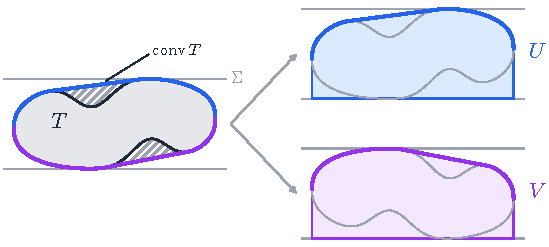
\includegraphics[width=.82\textwidth]{figures/fig-reduction.pdf}
 \caption{The original body $T$, its convex hull, and the two
 downward caps $U$ and $V$. The upper hull boundary is the roof of
 $U$; reflecting the lower hull boundary gives the roof of $V$.
 The hatched part illustrates area added by convexification.}
 \label{fig:reduction}
\end{figure}

Downward filling preserves support in every direction with
nonnegative vertical component. Since both $u(\theta)$ and
$u^\perp(\theta)$ point upwards for $0<\theta<\pi/2$, the
lower constraints of $T$ use exactly the supports of $U$. The
reflected upper constraints use those of $V$. Denote the resulting
barriers by
\[
 N_U=N_\alpha(U),\qquad N_V=N_\gamma(V).
\]
Each barrier includes the positive supremum of the two-wall minima
over the entire open angular interval and the terminal first wall
\[
 a_\alpha(x)=\frac{h_U(\alpha)-1-x\cos\alpha}{\sin\alpha}
\]
(with $V,\gamma$ for the other passage). This last wall is redundant
at a full quarter turn and is retained at every proper endpoint.
Thus every $(x,y)\in T$ satisfies $N_U(x)\le y$ and
$N_V(x)\le1-y$.



\runin{Physical fibers and the exact partition loss.}
Put $d_U=1-f_U$ and $d_V=1-f_V$. The actual four-wall envelope is
\begin{equation}\label{eq:physical-envelope}
 E=\left\{(x,y):x\in I,\quad
    \max\{d_V(x),N_U(x)\}\le y
    \le1-\max\{d_U(x),N_V(x)\}\right\}.
\end{equation}
We have $T\subseteq E$. Its signed fiber length is
\begin{equation}\label{eq:signed-length}
 \ell(x)=1-\max\{d_V(x),N_U(x)\}
             -\max\{d_U(x),N_V(x)\}.
\end{equation}
For arbitrary wall data, the actual length of that fiber is
$\ell(x)_+=\max\{\ell(x),0\}$. Here connectedness supplies a point
of $T$ at every $x\in I$, and containment supplies a point of $E$
in the same fiber. Consequently $\ell(x)\ge0$ everywhere on $I$,
and Cavalieri's formula gives
\begin{equation}\label{eq:envelope-area}
 |E|=\int_I\ell(x)\,\dd x\ge|T|.
\end{equation}
Compactness gives measurable roofs. The barriers are continuous by \cref{lem:barrier-continuity},
so all these functions are measurable and integrable on $I$.

Let $J=[l+w/4,r-w/4]=J_U=J_V$ be the middle half of $I$. Define
\begin{align}\label{eq:partition-defect}
 D_{\rm part}={}&
 \int_J\bigl[(d_V-N_U)_++(d_U-N_V)_+\bigr]\,\dd x\notag\\
 &+\int_{I\setminus J}
       \bigl[(N_U-d_V)_++(N_V-d_U)_+\bigr]\,\dd x.
\end{align}
It is nonnegative. The pointwise identity
$\max\{a,b\}-a=(b-a)_+$ yields
\[
 \begin{cases}
  1-N_U-N_V-\ell=(d_V-N_U)_++(d_U-N_V)_+,&x\in J,\\
  1-d_U-d_V-\ell=(N_U-d_V)_++(N_V-d_U)_+,&x\in I\setminus J.
 \end{cases}
\]
Since $|J|=|I\setminus J|=w/2$, the constant terms cancel on
integration. Recalling the score
\[
 P_\alpha(U)=\int_{I\setminus J}f_U\,\dd x
                         -\int_J N_U\,\dd x,
\]
we obtain the exact identity
\begin{equation}\label{eq:score-envelope-defect}
 P_\alpha(U)+P_\gamma(V)-|E|=D_{\rm part}.
\end{equation}

\begin{proposition}[Original-body score reduction]\label{prop:reduction}
Every ambidextrous sofa $S$ satisfies either $|S|\le\sqrt2$, or,
after an area-preserving rigid normalization, has the actual caps
$U,V$ and independent angles \eqref{eq:effective-angles} with
\begin{equation}\label{eq:two-cap-bound}
 |S|\le P_\alpha(U)+P_\gamma(V).
\end{equation}
More precisely, for every real comparison constant $c$,
\begin{equation}\label{eq:four-term-deficit}
 \begin{split}
 c-|S|={}&\left(\frac c2-P_\alpha(U)\right)
          +\left(\frac c2-P_\gamma(V)\right)\\
         &+D_{\rm part}+|E\setminus T|.
 \end{split}
\end{equation}
\end{proposition}

\begin{proof}
The small-area alternative is immediate. In the other case use the
normalization, effective-angle lemma, and actual cap constructions
above. The measurable bounded envelope contains $T$, so
$|E\setminus T|=|E|-|T|$. Substitute this into
\eqref{eq:score-envelope-defect}, then use $|T|=|S|$.
Dropping the two nonnegative geometric losses gives
\eqref{eq:two-cap-bound}.
\end{proof}

The scalar score in \cref{prop:reduction} is defined on every downward
cap, whether or not that cap arises from a feasible connected body.
The signed algebra also holds on that larger domain. The conversion
of $\int\ell$ into ordinary area used the actual body's connected
projection; it is needed only for the reduction from physical sofas.

\begin{remark}\label{rem:negative-fibers}
This distinction cannot be dropped for arbitrary convex hulls.
Take $K=[-1,1]\times[0,1]$ and both full angles. At $x=0$ the two
inner walls for $\theta=\pi/4$ have height $2-\sqrt2$.
Thus $N_U(0),N_V(0)\ge2-\sqrt2$, and
$\ell(0)\le2\sqrt2-3<0$. The central envelope fiber is empty.
The general area formula is $|E|=\int_I\ell_+\,\dd x$;
\eqref{eq:envelope-area} applies because the original connected body
certifies that every fiber is nonempty.
\end{remark}
